\documentclass[10.5pt,scale=1.0,t,aspectratio=169,hyperref={pdfpagelabels=false}]{beamer}


\usepackage{lipsum}
\usepackage{color}
\usepackage{amsfonts}
\usepackage{amsmath,mathtools}
\usepackage{mathrsfs}
\usepackage{array}
\usepackage{algorithm}
\usepackage{hyperref}
\usepackage[spanish,es-nodecimaldot]{babel}
\usepackage[utf8]{inputenc}
\usepackage{graphicx}
\usepackage{multicol}
\usepackage{multirow}
\usepackage{enumitem}
\usepackage[document]{ragged2e}
\usepackage[absolute,overlay]{textpos}
\textblockorigin{0mm}{0mm} 
\usefonttheme[onlymath]{serif}
\usepackage{verbatim}
\usepackage{cite}
\usepackage{multicol}
\usepackage{siunitx}




\newenvironment{conditions}[1][where:]
{#1 \begin{tabular}[t]{>{$}l<{$} @{${}={}$} l}}
	{\end{tabular}\\[\belowdisplayskip]}


\newcolumntype{L}{>{$}l<{$}} % math-mode version of "l" column type


\newcounter{saveenumi}
\newcommand{\seti}{\setcounter{saveenumi}{\value{enumi}}}
\newcommand{\conti}{\setcounter{enumi}{\value{saveenumi}}}

\setbeamertemplate{bibliography item}{\insertbiblabel}


\hypersetup{colorlinks=true,
	linkcolor=blue,
	linktoc=all,				
	citecolor=blue,
	urlcolor=red,
	pdftitle={DIGITAL CIRCUITS},
	pdfauthor={Santiago Rúa Pérez},
	pdfcreator={Santiago Rúa Pérez}}


\definecolor{GreenDark}{rgb}{0.0, 0.60, 0.0}
\definecolor{RedDark}{rgb}{183, 0.0, 0.0}
\definecolor{BlueDark}{rgb}{0.0, 0.0, 167}
\definecolor{BlueLight}{rgb}{0.2, 0.451, 0.517}


\graphicspath{{imag/}}

\newcommand{\Ho}{$H_{0}$}
\newcommand{\Ha}{$H_{a}$}
\newcommand{\Nota}{{\bf Nota: }}
\newcolumntype{P}[1]{>{\centering\arraybackslash}p{#1}}
\newcolumntype{M}[1]{>{\centering\arraybackslash}m{#1}}

\newcommand{\less}{<}
\newcommand{\greater}{>}


\setlength{\parindent}{1em}
\setlength{\parskip}{.6em}
\renewcommand{\baselinestretch}{.9}

%%%%    C environment    ---------------- %%%%%%%%%%%%%%%.
\usepackage{listings}
\usepackage{xcolor}
\definecolor{mGreen}{rgb}{0,0.6,0}
\definecolor{mGray}{rgb}{0.5,0.5,0.5}
\definecolor{mPurple}{rgb}{0.58,0,0.82}
\definecolor{backgroundColour}{rgb}{0.95,0.95,0.92}

\lstdefinestyle{CStyle}{
	backgroundcolor=\color{backgroundColour},   
	commentstyle=\color{mGreen},
	keywordstyle=\color{magenta},
	numberstyle=\tiny\color{mGray},
	stringstyle=\color{mPurple},
	basicstyle=\scriptsize,
	breakatwhitespace=false,         
	breaklines=true,                 
	captionpos=b,                    
	keepspaces=true,                 
	numbers=left,                    
	numbersep=5pt,                  
	showspaces=false,                
	showstringspaces=false,
	showtabs=false,                  
	tabsize=2,
	language=C
}
%%--------------------------------------------------------------------------


\title{Electrónica Digital II}   
\author{Santiago Rúa Pérez, PhD.} 
\date{\today} 

\setlength{\TPHorizModule}{\textwidth}
\setlength{\TPVertModule}{\textwidth}

\newcommand{\btVFill}{\vskip0pt plus 1filll}


\setbeamertemplate{sidebar right}{}
\setbeamertemplate{footline}
{
	\leavevmode%
	\hbox{%
		\begin{beamercolorbox}[wd=.333333\paperwidth,ht=2.25ex,dp=1ex,center]{author in head/foot}%
			\usebeamerfont{author in head/foot}\insertshortauthor
		\end{beamercolorbox}%
		\begin{beamercolorbox}[wd=.333333\paperwidth,ht=2.25ex,dp=1ex,center]{title in head/foot}%
			\usebeamerfont{title in head/foot}\insertshorttitle
	\end{beamercolorbox}}%
	\vskip0pt%
}
\makeatother

\begin{document}
	%%%%%%%%%%%%%%%%%% FRAME %%%%%%%%%%%%%%%%%%%%%%%%%%
	\begin{frame}
		\titlepage
	\end{frame}
	%%%%%%%%%%%%%%%%% FRAME START %%%%%%%%%%%%%%%%%%%%%%%%%%
	\frame{
		%\frametitle{}
		\begin{center}
			\LARGE \textcolor{blue}{TEMPORIZADORES}
		\end{center}
		
	}
	
	%%%%%%%%%%%%%%%%% FRAME %%%%%%%%%%%%%%%%%%%%%%%%%%

%%%%%%%%%%%%%%%%% FRAME %%%%%%%%%%%%%%%%%%%%%%%%%%
\begin{frame}
\frametitle{Objetivos}
\begin{itemize}
\item Entender como funciona el temporizador de todo procesador Cortex-M
\item Comprender el funcionamiento del PIT
\item Entender el funcionamiento del PWM
\end{itemize}
\end{frame}
%%%%%%%%%%%%%%%%% FRAME %%%%%%%%%%%%%%%%%%%%%%%%%%
\begin{frame}
	\frametitle{Temporizadores del K64}
	{\small
	\begin{columns}
		\column{0.5\linewidth}
		\begin{itemize}
			\item SYSTICK
			\begin{itemize}
				\item Parte de la CPU, y específicamente en la arquitectura Cortex-M
				\item Genera interrupción periódica
			\end{itemize}
			\item PIT - Periodic Interrupt Timer
			\begin{itemize}
				\item Puede ser generado periódicamente por interrupción o triggerear transferencia DMA (acceso directo a memoria)
			\end{itemize}
			\item FTM - FlexTimer/Módulo PWM 
			\begin{itemize}
				\item Conectarse a I/O pines y soportar captura de entrada y comparación de salida. 
				\item Puede generar se\~nales PWM
				\item Puede generar interrupciones y peticiones del DMA
			\end{itemize}
		\end{itemize}
	
		\column{0.5\linewidth}
		\begin{itemize}
			\item LPTMR - Low Power Timer
			\begin{itemize}
				\item Puede operar como temporizador o contador en todos los modos de potencia
				\item Puede despertar el sistema con interrupción
				\item Puede triggerear hardware. 
			\end{itemize}
			\item Real-Time Clock
			\begin{itemize}
				\item Energizado por cristal externo de \SI{32.768}{\kilo\hertz}32.768 kHz
				\item Mantiene dato del tiempo en registro de 32 bits
				\item Puede configurar alarma
				\item Puede generar se\~nal de \SI{1}{\hertz}
				\item Puede despertar el sistema
			\end{itemize}
		\end{itemize}
	\end{columns}
	}
\end{frame}
%%%%%%%%%%%%%%%%% FRAME %%%%%%%%%%%%%%%%%%%%%%%%%%
\begin{frame}
	\frametitle{Introduccion a los temporizadores y contadores }
	{\small
	\begin{figure}
		\centering
		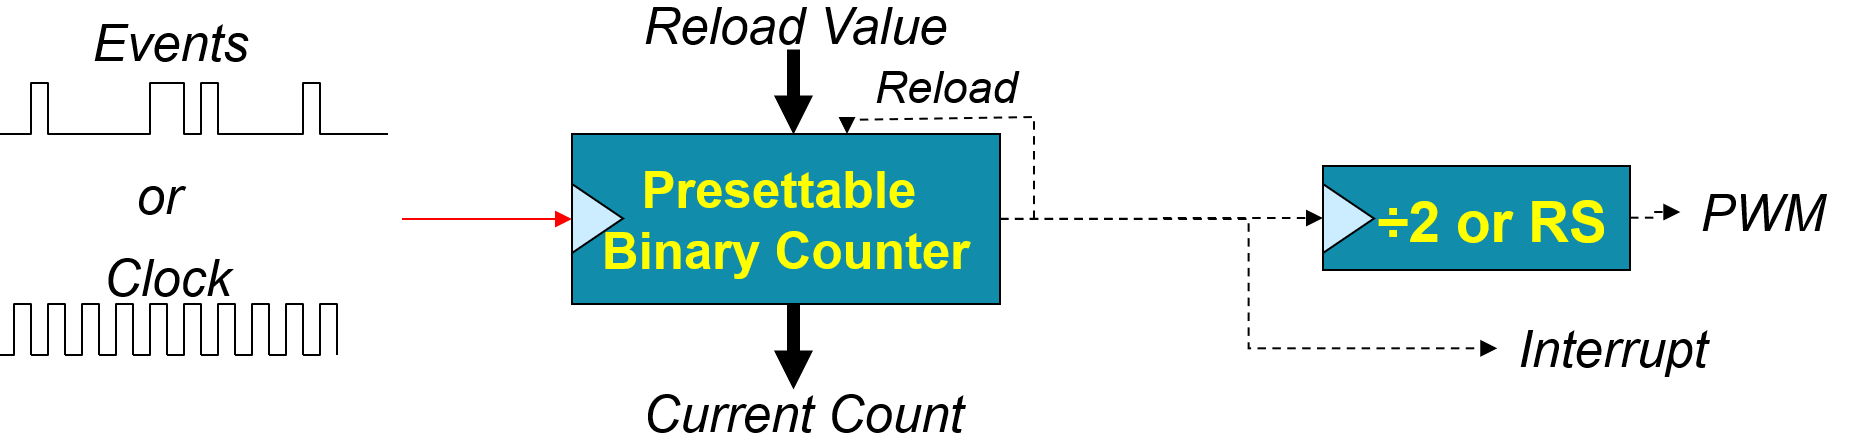
\includegraphics[scale=0.3]{01_GenericTimer}
	\end{figure}	
	\begin{columns}
		\column{0.6\linewidth}
		\begin{itemize}
			 \setlength\itemsep{0em}
			\item Es muy común en todos los microcontroladores
			\item Basado en un contador binario
			\item Dos modos básicos
			\begin{itemize}
				\item \textbf{Modo contador}: cuenta pulsos los cuales indican eventos (eg. odómetro)
				\item \textbf{Modo temporizador}: la fuente del reloj es periódica, entonces el valor del contador el proporcional al tiempo transcurrido.
			\end{itemize}
		\end{itemize}
	
		\column{0.4\linewidth}
		\begin{itemize}
			\item Principales configuraciones
			\begin{itemize}
				\item Valor del contador actual
				\item Valor de carga del contador
				\item Dirección de conteo
				\item Fuente del reloj
				\item Acciones de desbordamiento
			\end{itemize}
		\end{itemize}
	\end{columns}
	}
\end{frame}
%%%%%%%%%%%%%%%%% FRAME %%%%%%%%%%%%%%%%%%%%%%%%%%
\begin{frame}
	\frametitle{SysTick Timer }
	{\small
		\begin{columns}
			\column{0.5\linewidth}
			\begin{itemize}
				\item La arquitectura del procesador Cortex M contiene un temporizador integrado
				\item Contador de 24 bits en decremento. 
				\item Tiene cuatro registros (SysTick): CTRL, LOAD, VAL, y CALIB.
				\item Cuando se habilita el contador de 24 bits es cargado y cada pulso de reloj hace que decremente
				\item En el registro VAL se puede leer el valor actual del contador
				\item Se puede configurar su funcionamiento con el registro de control CTRL
				\begin{itemize}
					\item El CLKSOURCE define la fuente de reloj. Para el K64 está siempre conectado al core clock. 
				\end{itemize}
			\end{itemize}
			
			\column{0.5\linewidth}
			\begin{itemize}
				\item[] \begin{itemize}
					\item El TICKINT define si se activa la interrupción
					\item ENABLE habilita el contador con 1
					\item COUNTFLAG retorna 1 si el contador ha llegado a cero
				\end{itemize}
			\end{itemize}
			
		\end{columns}
	}
\end{frame}

%%%%%%%%%%%%%%%%% FRAME %%%%%%%%%%%%%%%%%%%%%%%%%%
\begin{frame}
	\frametitle{Ejemplo - SysTick Timer }
	{\small
		\begin{itemize}
			\item Realizar un programa que genere una interrupción del SysTick cada \SI{1}{\milli\second}. Adicionalmente, que togglee un led cada \SI{1}{\second}.
			\item \textbf{Solución}
			\begin{itemize}
				\item Inicialice el clock del procesador.
				\item Inicialice el GPIO como salida para el led.
				\item Configura el SysTick
				\item Escriba la función de atención a la interrupción
			\end{itemize}
		\end{itemize}
	
		\textbf{Nota 1}: la inicialización del clock del procesador se hará con el ayudante del MCU Expresso y específicamente del SDK del procesador. 
		
		\textbf{Nota 2}: el CMSIS-core nos presenta una función para la configuración del SysTick. Activa de una vez la interrupción. 
		
		\hspace{2cm} \texttt{\_\_STATIC\_INLINE uint32\_t SysTick\_Config(uint32\_t ticks)}	
	}
\end{frame}

%%%%%%%%%%%%%%%%% FRAME %%%%%%%%%%%%%%%%%%%%%%%%%%
\begin{frame}[fragile]
	\frametitle{Ejemplo - SysTick Timer }
	{\small
		\begin{itemize}
			\item Inicializacion del rgb.
			\begin{lstlisting}[style=CStyle]
#define LED_BLUE 21
#define MASK(x) (1UL << (x))

void init_rgb(void);
				
void init_rgb(void){
	SIM->SCGC5 |= SIM_SCGC5_PORTB_MASK; //| SIM_SCGC5_PORTC_MASK;
	PORTB->PCR[LED_BLUE] = PORT_PCR_MUX(1);
	PTB->PDDR |= MASK(LED_BLUE);
	PTB->PCOR |= MASK(LED_BLUE);
}
			\end{lstlisting}
		\item ISR SysTick.
		\begin{lstlisting}[style=CStyle]
void SysTick_Handler(void){
	band++;
}
		\end{lstlisting}
		\end{itemize}
	}
\end{frame}

%%%%%%%%%%%%%%%%% FRAME %%%%%%%%%%%%%%%%%%%%%%%%%%
\begin{frame}[fragile]
	\frametitle{Ejemplo - SysTick Timer }
	{\small
		\begin{itemize}
			\item Main.
			\begin{lstlisting}[style=CStyle]
int main(void) {
	/* Init board hardware. */
	BOARD_InitBootClocks();
	init_rgb();
	/* Init SysTick to 120000 of ticks = 1 ms */
	SysTick_Config(120000UL);
	while(1) {
		if(band>=1000){
			PTB->PTOR |= MASK(LED_BLUE);
			band = 0;
		}
	}
	return 0;
}
			\end{lstlisting}
		\end{itemize}
	}

\textbf{Limitaciones}: solo cuenta con uno y de 24 bits. Decrementa. 
\end{frame}

%%%%%%%%%%%%%%%%% FRAME %%%%%%%%%%%%%%%%%%%%%%%%%%
\begin{frame}
	\frametitle{Periodic Interrupt Timmer - PIT }
	{\small
		\begin{columns}
			\column{0.5\linewidth}
			\begin{figure}
				\centering
				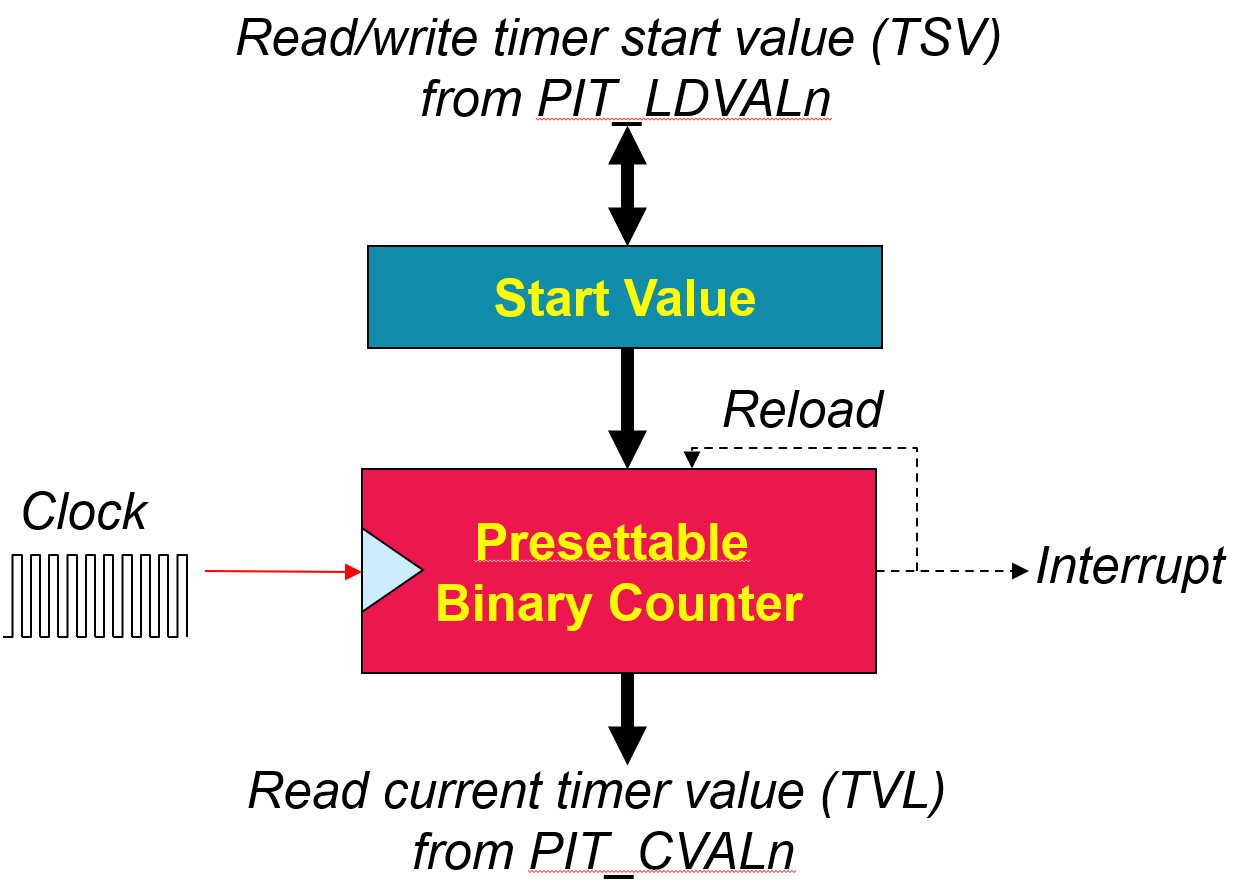
\includegraphics[scale=0.3]{02_PIT}
			\end{figure}
		
			\column{0.5\linewidth}
			\begin{itemize}
				\item Genera una interrupción periodica usando contador de 32 bits
				\item Se carga el valor inicial en el registro LDVAL
				\item Contador decrementa con cada pulso del reloj
				\begin{itemize}
					\item Fuente de reloj fija para el PIT - Clock del Bus. 
				\end{itemize}
				\item Cuando el temporizador llega a cero (CVAL)
				\begin{itemize}
					\item Genera interrupción
					\item Carga el temporizador de nuevo con el valor inicial
				\end{itemize}
			\end{itemize}
		\end{columns}
	}
\end{frame}

%%%%%%%%%%%%%%%%% FRAME %%%%%%%%%%%%%%%%%%%%%%%%%%
\begin{frame}
	\frametitle{PIT Diagrama de tiempo}
	{\small
	\begin{figure}
		\centering
		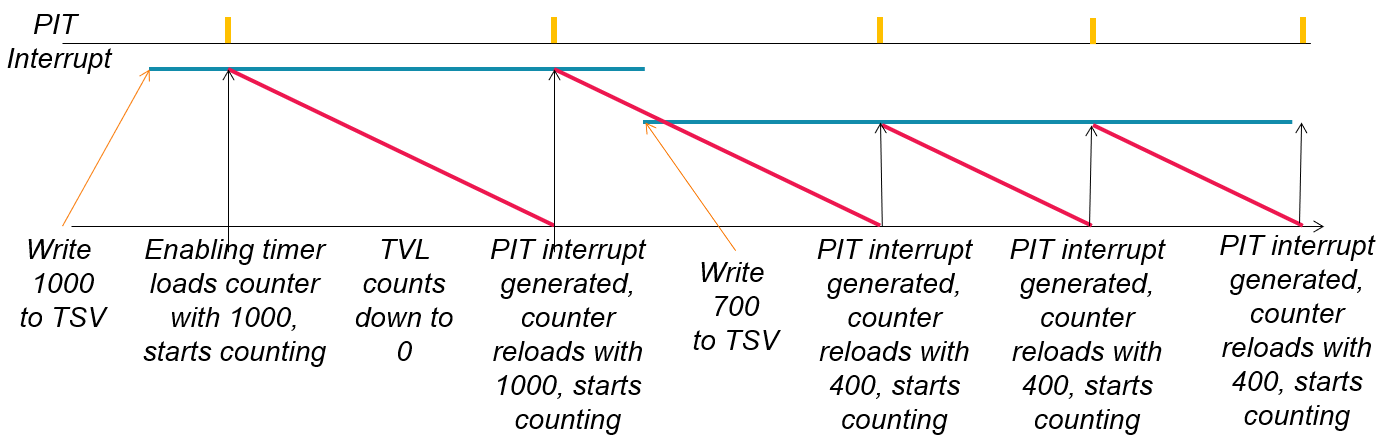
\includegraphics[scale=0.6]{03_PITDiagramTime}
	\end{figure}
		
		\textbf{Nota}: solo se actualiza el valor hasta que termina de contar completamente. 	
	}
\end{frame}

%%%%%%%%%%%%%%%%% FRAME %%%%%%%%%%%%%%%%%%%%%%%%%%
\begin{frame}
	\frametitle{Configuración del PIT }
	{\small
		\begin{columns}
			\column{0.5\linewidth}
			\begin{itemize}
				\item Habilitar el clock del periférico
				\begin{itemize}
					\item SIMCGC6 PIT
				\end{itemize}
				\item Registro de control del módulo (PIT-$>$MCR)
				\begin{itemize}
					\item MDIS - 0: habilitado, 1: deshabilitado
				\end{itemize}
				\item FRZ - stop timmer in debug
				\begin{itemize}
					\item 0: timmer corre en debug
					\item 1: timmer parados
				\end{itemize}
				\item Múltiples canales en el PIT. Para el k64 tiene 4 canales
				\item Puede hacer cadena de contadores para aumentar la capacidad. 
			\end{itemize}
			
			\column{0.5\linewidth}
			\begin{figure}
				\centering
				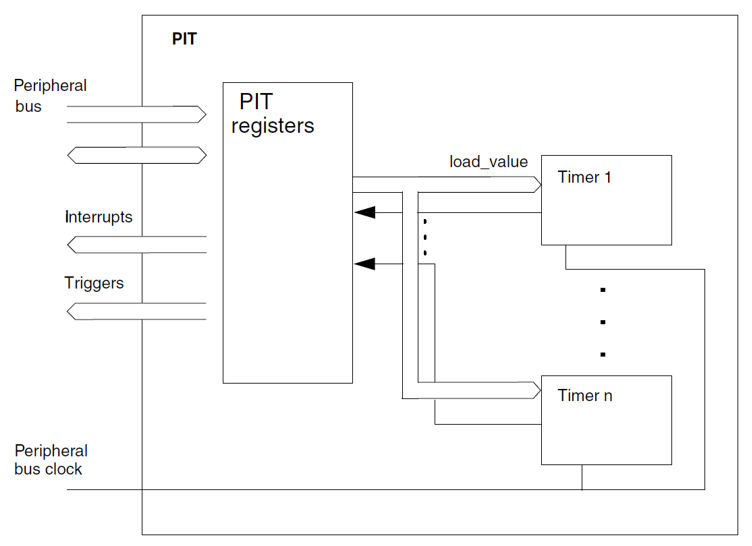
\includegraphics[scale=0.5]{04_PITHardware}
			\end{figure}
		\end{columns}
	}
\end{frame}
%%%%%%%%%%%%%%%%% FRAME %%%%%%%%%%%%%%%%%%%%%%%%%%
\begin{frame}
	\frametitle{Control de cada canal }
	{\small
		\begin{columns}
			\column{0.5\linewidth}
			\begin{itemize}
				\item  Interfaz CMSIS
				\begin{itemize}
					\item Acceso general con la estructura PIT-$>$MCR
					\item Los canales son accedidos como vectores de estructuras: PIT-$>$CHANNEL[n].LDVAL
				\end{itemize}
				\item PIT-$>$CHANNEL[n].LDVAL para cargar el valor
				\item PIT-$>$CHANNEL[n].CVAL valor actual del contador
				\item PIT-$>$CHANNEL[n].TCTRL registro de control
				\begin{itemize}
					\item CHN: 0 como independiente, 1 como cadena el cual cambia por el timer n-1
				\end{itemize}
			\end{itemize}
			
			\column{0.5\linewidth}
			\begin{itemize}
				\item[] \begin{itemize}
					\item TIE: habilita la interrupción. 0 no se habilita, 1 si.
					\item TEN: habilita el conteo. 0 comienza el conteo, 1 no cuenta.
					\item PIT\_TFLGn: bandera del timer. 1 es porque el tiempo se ha alcanzado. 
				\end{itemize}
			\end{itemize}
			
		\end{columns}
	}
\end{frame}
%%%%%%%%%%%%%%%%% FRAME %%%%%%%%%%%%%%%%%%%%%%%%%%
\begin{frame}[fragile]
	\frametitle{Configurando el PIT}
	{\small
		\begin{itemize}
			\setlength\itemsep{0em}
			\item Habilitar el clock del PIT
			\begin{lstlisting}[style=CStyle]
SIM->SCGC6 |= SIM_SCGC6_PIT_MASK;				
			\end{lstlisting}
			\item Habilita el modulo, congela el timer mientras DEBUG
			\begin{lstlisting}[style=CStyle]
PIT->MCR &= ~PIT_MCR_MDIS_MASK;
PIT->MCR |= PIT_MCR_FRZ_MASK;			
			\end{lstlisting}
			\item Inicializa el PIT para contar en forma descendiente.
			\begin{lstlisting}[style=CStyle]
PIT->CHANNEL[channel].LDVAL = PIT_LDVAL_TSV(TimeValue); // 60 MHz
			\end{lstlisting}
			\item No se hace cadena de timmers y no se habiita por el momento el PIT
			\begin{lstlisting}[style=CStyle]
PIT->CHANNEL[channel].TCTRL &= ~PIT_TCTRL_CHN_MASK & ~PIT_TCTRL_TEN_MASK;			
			\end{lstlisting}
		\end{itemize}
	}
\end{frame}

%%%%%%%%%%%%%%%%% FRAME %%%%%%%%%%%%%%%%%%%%%%%%%%
\begin{frame}[fragile]
	\frametitle{Obteniendo el valor de carga}
	{\small
		\begin{itemize}
			\setlength\itemsep{0em}
			\item Meta: generar una interrupcion cada T segundos
			\item LDVAL: redondeo($T * f_{count} - 1$)
			\begin{itemize}
				\item -1 ya que el contador va hasta cero.
				\item Redondear ya que es entero el registro. 
			\end{itemize}
			\item \textbf{Ejemplo}: Interrupción cada \SI{137.41}{\milli\second}
			\begin{itemize}
				\item LDVAL $=\SI{137.41}{\milli\second} * \SI{24}{\mega\hertz} - 1 = 3297839$
			\end{itemize}
			\item \textbf{Ejemplo}: Interrupción con frecuencia de  \SI{91}{\hertz}
			\begin{itemize}
				\item LDVAL $=1/\SI{91}{\hertz} * \SI{24}{\mega\hertz} - 1 = 263734$
			\end{itemize}
		\end{itemize}
	}
\end{frame}
%%%%%%%%%%%%%%%%% FRAME %%%%%%%%%%%%%%%%%%%%%%%%%%
\begin{frame}[fragile]
	\frametitle{Configurando las interrupciones del PIT}
	{\small
		\begin{itemize}
			\setlength\itemsep{0em}
			\item Configure el PIT
			\begin{lstlisting}[style=CStyle]
PIT->CHANNEL[channel].TCTRL |= PIT_TCTRL_TIE_MASK;			
			\end{lstlisting}
			\item Configure el NVIC
			\begin{itemize}
				\item Configure la prioridad
				\item Limpie cualquier IRQ del PIT pendiente.
				\item Habilite la interrupción
				\begin{lstlisting}[style=CStyle]
PIT->CHANNEL[channel].TCTRL |= PIT_TCTRL_TIE_MASK;
NVIC_SetPriority(PIT0_IRQn+channel, 64); // 0, 64, 128 or 192
NVIC_ClearPendingIRQ(PIT0_IRQn+channel);
NVIC_EnableIRQ(PIT0_IRQn+channel);		
				\end{lstlisting}
			\end{itemize}
		
			\item Asegúrese que las interrupciones no estén enmascaradas globalmente. 
			\begin{lstlisting}[style=CStyle]
__enable_irq();	
			\end{lstlisting}
		\end{itemize}
	}
\end{frame}
%%%%%%%%%%%%%%%%% FRAME %%%%%%%%%%%%%%%%%%%%%%%%%%
\begin{frame}
	\frametitle{Handler de la interrupción}
	{\small
		\begin{itemize}
			\setlength\itemsep{0em}
			\item Una función de atención a interrupción por cada canal
			\item Nombre del CMSIS
			\begin{itemize}
				\item \texttt{void PIT0\_IRQHandler(void)}
				\item \texttt{void PIT1\_IRQHandler(void)}
				\item \texttt{void PIT2\_IRQHandler(void)}
				\item \texttt{void PIT3\_IRQHandler(void)}
			\end{itemize}
			\item Actividades dentro del ISR
			\begin{itemize}
				\item Determinar cual canal genero la interrupción. 
				
				\texttt{if (PIT-$>$CHANNEL[0].TFLG \& PIT\_TFLG\_TIF\_MASK)}
				\item Limpiar la interrupción. 
				
				\texttt{IT-$>$CHANNEL[0].TFLG \&= PIT\_TFLG\_TIF\_MASK;}
				\item Hacer la tarea del ISR
			\end{itemize}
		\end{itemize}
	}
\end{frame}
%%%%%%%%%%%%%%%%% FRAME %%%%%%%%%%%%%%%%%%%%%%%%%%
\begin{frame}
	\frametitle{Iniciar y parar el timer}
	{\small
		\begin{itemize}
			\setlength\itemsep{0em}
			\item Iniciar el timer
			
			\texttt{PIT-$>$CHANNEL[0].TCTRL |= PIT\_TCTRL\_TEN\_MASK;}
			
			\item Parar el timer
			
			\texttt{PIT-$>$CHANNEL[0].TCTRL \&= ~PIT\_TCTRL\_TEN\_MASK;}
		\end{itemize}
	}
\end{frame}
%%%%%%%%%%%%%%%%% FRAME %%%%%%%%%%%%%%%%%%%%%%%%%%
\begin{frame}
	\frametitle{Ejemplo PIT}
	{\small
		Hacer un programa que genere una interrupción cada \SI{1}{\second}. Una vez se presione el pulsador, el led comienza a parpadear cada segundo. El led debe parpadear 10 veces y luego parar. El parpadeo inicia de nuevo cuando se presiona el pulsador. 
		
		\textbf{Solución}:
		
		\begin{itemize}
			\item Inicializar los clock
			\item Inicializar el pulsador
			\item Inicializar el rgb
			\item Inicializar el PIT
			\item Tener en cuenta las interrupciones tanto del pulsador como del PIT.
		\end{itemize}
	}
\end{frame}
%%%%%%%%%%%%%%%%% FRAME %%%%%%%%%%%%%%%%%%%%%%%%%%
\begin{frame}[fragile]
	\frametitle{Ejemplo PIT - Solución}
	{\small
\begin{lstlisting}[style=CStyle]
void Init_PIT(uint8_t channel, unsigned period_us, uint8_t gen_interrupts) {
	// Enable clock to PIT module
	SIM->SCGC6 |= SIM_SCGC6_PIT_MASK;
	
	// Enable module, freeze timers in debug mode
	PIT->MCR &= ~PIT_MCR_MDIS_MASK;
	PIT->MCR |= PIT_MCR_FRZ_MASK;
	
	// Initialize PIT to count down from argument
	PIT->CHANNEL[channel].LDVAL = PIT_LDVAL_TSV((period_us*60)-1); // 60 MHz bus 
	
	// No chaining
	PIT->CHANNEL[channel].TCTRL &= PIT_TCTRL_CHN_MASK;
	
	if (gen_interrupts) {
		// Generate interrupts
		PIT->CHANNEL[channel].TCTRL |= PIT_TCTRL_TIE_MASK;
		// Configure NVIC
		NVIC_SetPriority(PIT0_IRQn+channel, 64); // 0, 64, 128 or 192
		NVIC_ClearPendingIRQ(PIT0_IRQn+channel);
		NVIC_EnableIRQ(PIT0_IRQn+channel);
	}
}
\end{lstlisting}		
	}
\end{frame}
%%%%%%%%%%%%%%%%% FRAME %%%%%%%%%%%%%%%%%%%%%%%%%%
\begin{frame}[fragile]
	\frametitle{Ejemplo PIT - Solución}
	{\small
		\begin{lstlisting}[style=CStyle]
void Start_PIT(uint8_t channel) {
	// Enable counter
	PIT->CHANNEL[channel].TCTRL |= PIT_TCTRL_TEN_MASK;
}

void Stop_PIT(uint8_t channel) {
	// Disable counter
	PIT->CHANNEL[channel].TCTRL &= ~PIT_TCTRL_TEN_MASK;
}

void PIT0_IRQHandler(void){
	// check to see which channel triggered interrupt
	if (PIT->CHANNEL[0].TFLG & PIT_TFLG_TIF_MASK) {
		// clear status flag for timer channel 0
		PIT->CHANNEL[0].TFLG &= PIT_TFLG_TIF_MASK;
		bandPIT = 1;
		PTE->PTOR |= MASK(LED_GREEN);
	}
}
		\end{lstlisting}		
	}
\end{frame}
%%%%%%%%%%%%%%%%% FRAME %%%%%%%%%%%%%%%%%%%%%%%%%%
\begin{frame}[fragile]
	\frametitle{Laboratorio 10\%}
	{\small
		Realizar el programa de las maquinas de estado para parpadear tanto led RGB como blanco y negro. Esta vez deberá realizar el delay con interrupción y no bloqueantes. Adicionalmente, los pulsadores tambien deberan tener interrupciones. Solo debe quedar el programa principal con dos tareas: la maquina de estados del RGB y la de Blanco y negro. 
		
		Adicionalmente, tendrá otra tercera tarea que se encarga de leer el valor de un potenciometro. El objetivo es que con dicho valor del potenciometro se cambie la intensidad de brillo de los leds. 		
	}
\end{frame}
%%%%%%%%%%%%%%%%% FRAME %%%%%%%%%%%%%%%%%%%%%%%%%%
\begin{frame}
	\frametitle{FlexTimer FTM / PMW}
	\vspace{-0.3cm}
	{\footnotesize
		\begin{columns}
			\column{0.6\linewidth}
			\begin{itemize}
				\setlength\itemsep{0em}
				\item Core: contador
				\begin{itemize}
					\item Diferentes opciones de reloj.
					\item Se puede escalar el reloj por 1 hasta 128
					\item Contador de 16-bit
					\begin{itemize}
						\item Puede contar ascendente o ascendente/descendente
						\item Se puede cargar el valor del contador
					\end{itemize}
				\end{itemize}
				\item Hasta 4 FTM con múltiples canales independientes (hasta 8)
				\begin{itemize}
					\item 3 modos
					\begin{itemize}
						\item Modo de captura: captura la señal de tiempo cuando la entrada cambia
						\item Comparación de salida: cambia la señal de salida cuando el temporizador alcanza cierto valor
						\item PWM: genera una señal por modulación de ancho de pulso.
					\end{itemize}
					\item Cada canal puede generar interrupcion, peticion DMA
					\item Un pin I/O por canal: FTMx\_CHn
				\end{itemize}
			\end{itemize}
		
			\column{0.4\linewidth}
			\begin{figure}
				\centering
				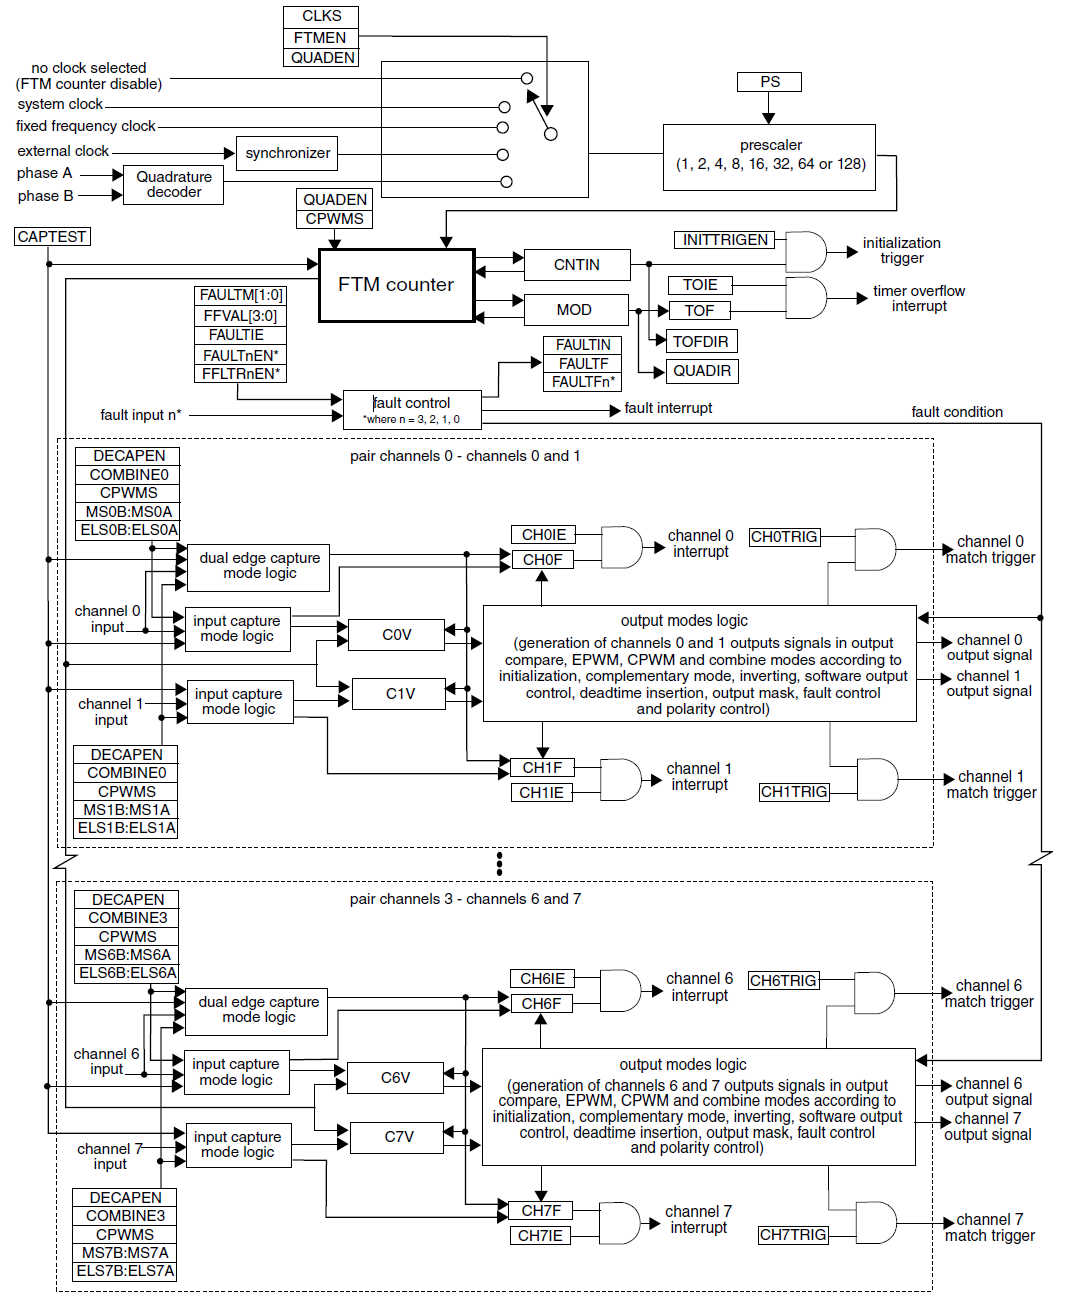
\includegraphics[scale=0.28]{05_PWMArchitecture}
			\end{figure}
		
		\end{columns}
	}
\end{frame}
%%%%%%%%%%%%%%%%% FRAME %%%%%%%%%%%%%%%%%%%%%%%%%%
\begin{frame}
	\frametitle{Configuración del FTM}
	\vspace{-0.3cm}
	{\footnotesize
		\begin{figure}
			\centering
			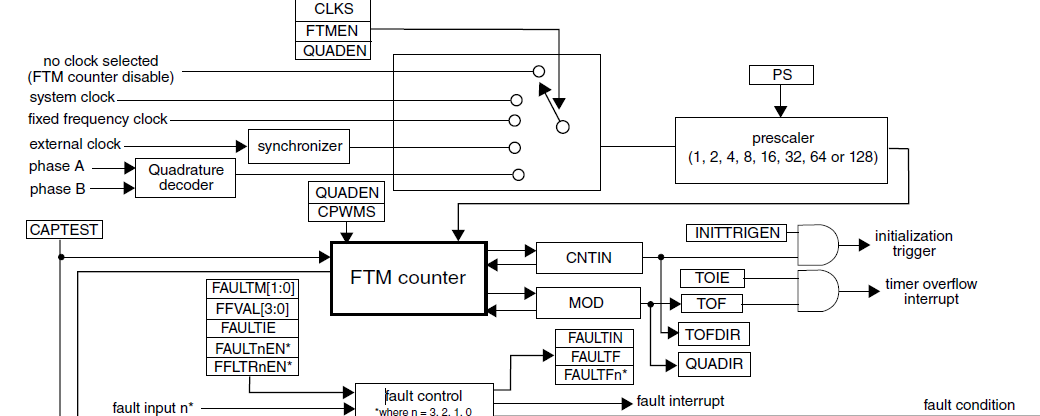
\includegraphics[scale=0.4]{06_TimerConfig}
		\end{figure}
	
		\begin{columns}
			\column{0.5\linewidth}
			\begin{itemize}
				\item Fuente de reloj
				\begin{itemize}
					\item CLKS: no clock, clock del sistema, clock de frecuencia fija o clock externo
				\end{itemize}
				\item Prescaler
				\begin{itemize}
					\item PS: divide el clock por 1, 2, 4, 8, 16, 32,64, 128
				\end{itemize}
				\item Modo de conteo
				\begin{itemize}
					\item CPWMS: conteo arriba (0) or arriba \& abajo (1)
				\end{itemize}
			\end{itemize}
		
			\column{0.5\linewidth}
			\begin{itemize}
				\item Módulo de conteo
				\begin{itemize}
					\item MOD: 16-bit
					\item Timer overflow cuando pasa dicho valor
					\item Conteo ascendente: 0, 1, ... MOD, 0/Overflow, 1, ...
					\item Up/down: 0, 1 ... MOD, MOD-1/ Interrupt, MOD-2, ..., 1, 0, 1, 2 ...
				\end{itemize}
				\item TOF: bandera que indica el temporizador a finalizado
			\end{itemize}
		\end{columns}
	}
\end{frame}
%%%%%%%%%%%%%%%%% FRAME %%%%%%%%%%%%%%%%%%%%%%%%%%
\begin{frame}
	\frametitle{Configuración como contador básico}
	\vspace{-0.3cm}
	{\footnotesize
		\begin{figure}
			\centering
			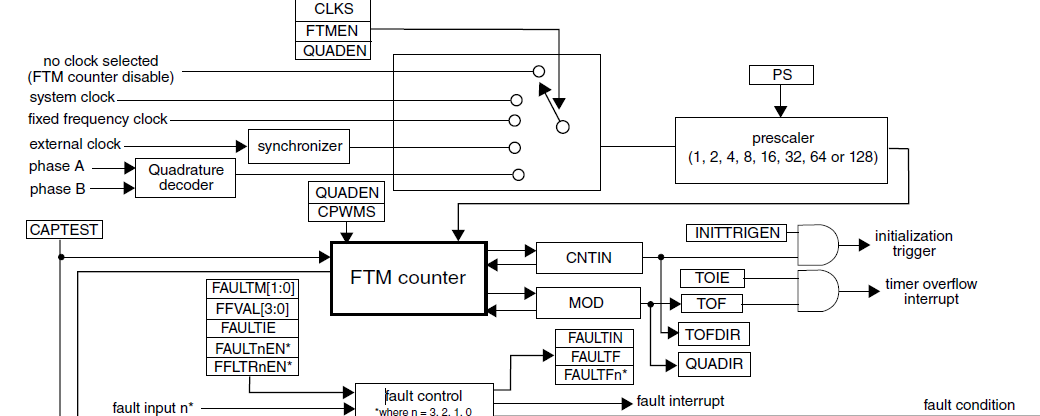
\includegraphics[scale=0.4]{06_TimerConfig}
		\end{figure}
		
		\begin{columns}
			\column{0.5\linewidth}
			\begin{itemize}
				\item Contar los evento externos aplicados al pin
				\begin{itemize}
					\item Poner CLKS=11 para seleccionar contador externo
					\item Poner PS=000 a no ser que se necesite división. 
				\end{itemize}
				\item La bandera de desbordamiento TOF se pone en 1 hasta recibir la cantidad de pulsos MOD
				\item Puede generar interrupción si TOIE está activada
			\end{itemize}
			
			\column{0.5\linewidth}
			\begin{table}[h]
				\begin{tabular}{cc}
				\hline
				\textbf{2-0 PS}	& \textbf{Prescaler Factor}  \\
				\hline
				000	& 1   \\
				001	& 2   \\
				010	& 4 \\
				011	& 8 \\
				100	& 16 \\
				101	& 32 \\
				110	& 64 \\
				111	& 128 \\
				\hline
				\end{tabular}
			\end{table}
		\end{columns}
	}
\end{frame}
%%%%%%%%%%%%%%%%% FRAME %%%%%%%%%%%%%%%%%%%%%%%%%%
\begin{frame}
	\frametitle{Modo de conteo - Conteo Ascendente}
	\vspace{-0.3cm}
	{\footnotesize
		\begin{figure}
			\centering
			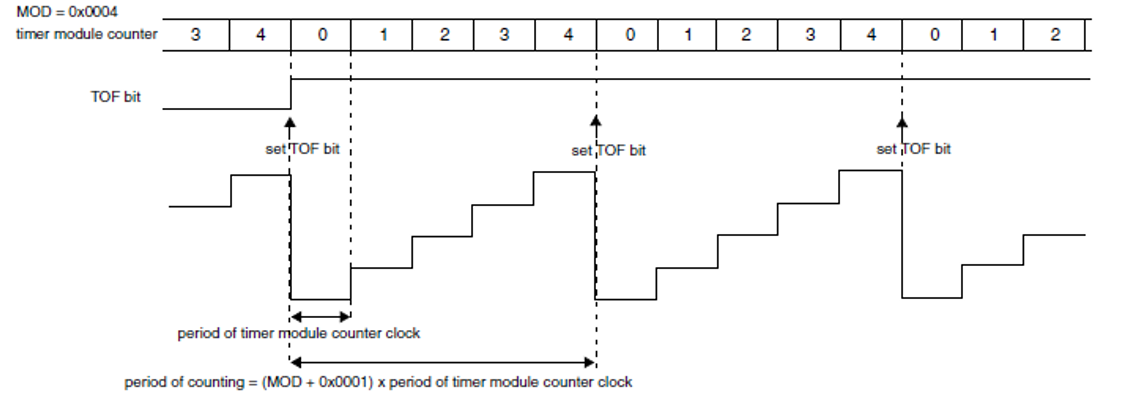
\includegraphics[scale=0.65]{07_CountingUp}
		\end{figure}
		
		\begin{columns}
			\column{0.5\linewidth}
			\begin{itemize}
				\item Contador incrementa con cada clock
				\item Cuando el contador llega al MOD
				\begin{itemize}
					\item Poner TOF en 1
					\item Resetea el valor a cero.
				\end{itemize}
			\end{itemize}
			
			\column{0.5\linewidth}
			\begin{itemize}
				\item La frecuencia será: frecuencia del timer/(1+MOD)
			\end{itemize}
		
		\end{columns}
	}
\end{frame}
%%%%%%%%%%%%%%%%% FRAME %%%%%%%%%%%%%%%%%%%%%%%%%%
\begin{frame}
	\frametitle{Modo de conteo - Conteo Ascendente/Descendente}
	\vspace{-0.3cm}
	{\footnotesize
		\begin{figure}
			\centering
			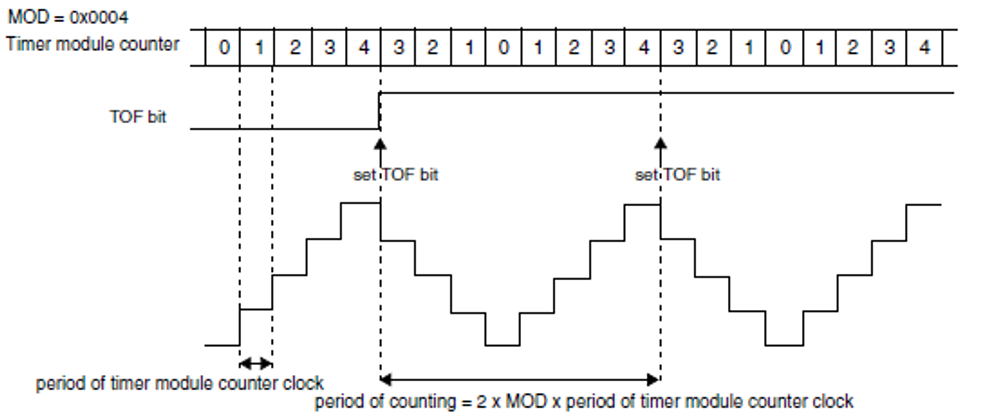
\includegraphics[scale=0.65]{08_CountingUpDown}
		\end{figure}
		
		\begin{columns}
			\column{0.5\linewidth}
			\begin{itemize}
				\item Fase ascendente
				\begin{itemize}
					\item Contador incrementa con cada clock
					\item Cuando llega al MOD, pone uno en TOF, y pasa a modo descendente
				\end{itemize}
			\end{itemize}
			
			\column{0.5\linewidth}
			\begin{itemize}
				\item Conteo descendente
				\begin{itemize}
					\item Contador decrementa con cada clock
					\item Cuando alcanza a cero, se pasa a modo ascendente.
				\end{itemize}
				\item La frecuencia de desbordamiento es: clock/(2*MOD)
			\end{itemize}
			
		\end{columns}
	}
\end{frame}
%%%%%%%%%%%%%%%%% FRAME %%%%%%%%%%%%%%%%%%%%%%%%%%
\begin{frame}
	\frametitle{Configuración del canal y valor}
	\vspace{-0.3cm}
	{\footnotesize
		\begin{columns}
			\column{0.4\linewidth}
			\begin{itemize}
				\item Configuración: FTMx\_CnSC
				\begin{itemize}
					\item CHF: ha ocurrido un evento (1) o no (0)
					\item CHIE: habilita el canal para generar interrupción
					\item MSB:MSA selección del modo
					\item ELSB:ELSA selección por flanco o nivel
					\item DMA
				\end{itemize}
				\item Valor: FTMx\_CnV
				\begin{itemize}
					\item Valor de salida de 16-bit.
				\end{itemize}
				\item El CMSIS agrupa estos dos campos es una estructura llamada CONTROLS para cada canal
				\begin{itemize}
					\item \texttt{FTM0-$>$CONTROLS[0].CnSC}
				\end{itemize}
			\end{itemize}
		
			\column{0.6\linewidth}
			{\tiny
			\begin{table}[]
				\begin{tabular}{ccccp{2cm}}
					\hline
					\textbf{CPWMS} & \textbf{MSnB:A} & \textbf{ELSnB:A} & \textbf{Modo} & \textbf{Config} \\
					\hline
					\multirow{3}{*}{0} & \multirow{3}{*}{00}      & 01 & \multirow{3}{*}{Input Capture} & Captura Flanco de subida   \\
					& & 10 &                       & Captura Flanco de bajada   \\
					& & 11 &                       & Captura ambos flancos  \\
					\hline
					\multirow{3}{*}{0} & \multirow{3}{*}{01}      & 01 & \multirow{3}{*}{Output Capture} & Toggle ouput on match   \\
					& & 10 &                       & Clear ouput on match   \\
					& & 11 &                       & Set ouput on match  \\
					\hline
					\multirow{2}{*}{0} & \multirow{2}{*}{1X}      & 10 & \multirow{2}{*}{Edge-Aligned
						PWM} & High-true pulses (clear Output on match)   \\
					& & X1 &   & Low-true pulses (set Output on
					match) \\
					\hline
					\multirow{2}{*}{1} & \multirow{2}{*}{XX}      & 10 & \multirow{2}{*}{Center-Aligned
						PWM} & High-true pulses (clear Output on match)   \\
					& & X1 &   & Low-true pulses (set Output on
					match) \\
					\hline
				\end{tabular}
			\end{table}
			}
		\end{columns}	
	}
\end{frame}
%%%%%%%%%%%%%%%%% FRAME %%%%%%%%%%%%%%%%%%%%%%%%%%
\begin{frame}
	\frametitle{Modulación por ancho de pulso}
	\vspace{-0.3cm}
	{\footnotesize
		\begin{columns}
			\column{0.6\linewidth}
			\begin{itemize}
				\item Posibilita una señal digital mandar dos valores 0,1.
				\item Facil codificación: valor es una fracción del tiempo.
				\item La señal puede ser promediada para crear una señal analógica.
				\item PWM características
				\begin{itemize}
					\item Modulación en frecuencia - cuantos pulsos ocurren en un segundo
					\item Periodo
					\item On-time - Cantidad de tiempo que el pulso esta activo
					\item Duty-cycle - on-time/periodo
					\item Configurar on-time para representar un valor análogo. 
				\end{itemize}
			\end{itemize}
			
			\column{0.4\linewidth}
			\begin{figure}
				\centering
				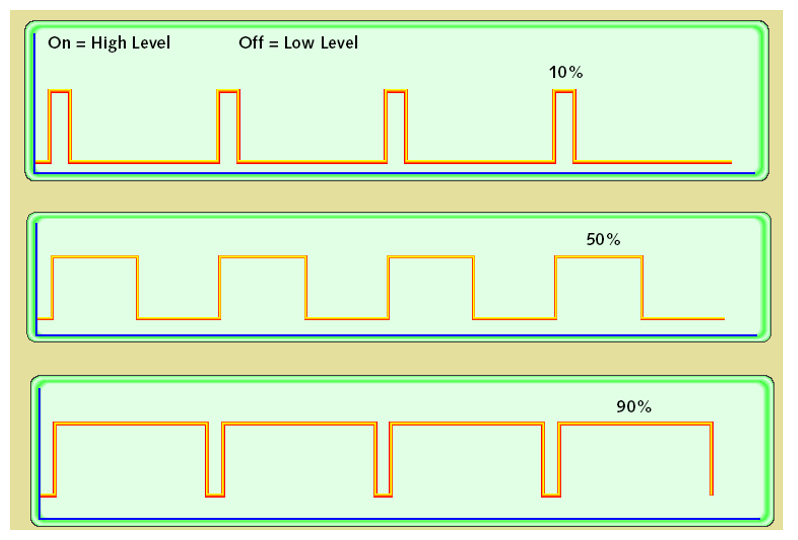
\includegraphics[scale=0.4]{09_PWMSignal}
			\end{figure}
			
		\end{columns}
	}
\end{frame}
%%%%%%%%%%%%%%%%% FRAME %%%%%%%%%%%%%%%%%%%%%%%%%%
\begin{frame}
	\frametitle{Modulación por ancho de pulso}
	\vspace{-0.3cm}
	{\footnotesize
		\begin{itemize}
			\item \textbf{Comunicaciones digitales}: es menos sensible al ruido que los métodos análogos. 
			\begin{itemize}
				\item PWM da una codificación digital para un valor análogo
				\item Menos vulnerable al ruido
			\end{itemize}
			\item \textbf{Amplificadores de potencia digitales}: son mas eficiente y menos costosos que los análogos. 
			\begin{itemize}
				\item Aplicaciones: control de velocidad deun motor, dimerizado de luces, conversión de potencia.
				\item Carga responde lentos, señal promedio. 
			\end{itemize}
		\end{itemize}
	}
\end{frame}
%%%%%%%%%%%%%%%%% FRAME %%%%%%%%%%%%%%%%%%%%%%%%%%
\begin{frame}
	\frametitle{Ejemplo - PWM}
	\vspace{-0.3cm}
	{\footnotesize
		Hacer que un led se dimerice cada tiempo yendo de total intensidad hasta apagarse. Volver a repetirse
		
		Solución:
		
		\begin{itemize}
			\item Inicializar los clock del procesador.
			\item Inicializar el FTM
			\begin{itemize}
				\item Activar el clock del puerto
				\item Activar el clock del FTM
				\item Poner el PCR en la alternativa de FTM
				\item Poner el modulo de conteo
				\item Seleccionar el preescaler
				\item Seleccionar el modo de operación (PWN alineado con flanco)
				\item poner el valor del duty-cycle
				\item Activar el clock del PWM
			\end{itemize}
		\end{itemize}
	}
\end{frame}
%%%%%%%%%%%%%%%%% FRAME %%%%%%%%%%%%%%%%%%%%%%%%%%
\begin{frame}[fragile]
	\frametitle{Ejemplo - Solución}
	\vspace{-0.2cm}
	{\footnotesize
	\begin{lstlisting}[style=CStyle]
void Init_Green_LED_PWM(uint16_t period){
	// Enable clock to port C
	SIM->SCGC5 |= SIM_SCGC5_PORTC_MASK;;
	
	// Blue FTM0_CH0, Mux Alt 4
	PORTC->PCR[LED_GREEN] &= ~PORT_PCR_MUX_MASK;
	PORTC->PCR[LED_GREEN] |= PORT_PCR_MUX(4);
	
	// Configure TPM
	SIM->SCGC6 |= SIM_SCGC6_FTM0_MASK;
	
	//load the counter and mod
	FTM0->MOD = period-1;
	
	//set TPM count direction to up (CPWMS = 0), Disable TOF interrupt, No clock selected, divide by 2 prescaler
	FTM0->SC =  FTM_SC_PS(2);
	
	// Set channel 0 to edge-aligned low-true PWM
	FTM0->CONTROLS[0].CnSC = FTM_CnSC_MSB_MASK | FTM_CnSC_ELSA_MASK;
	// Set initial duty cycle
	FTM0->CONTROLS[0].CnV = 0;
	// Start TPM
	FTM0->SC |= FTM_SC_CLKS(1);
}
	\end{lstlisting}
	}
\end{frame}
%%%%%%%%%%%%%%%%% FRAME %%%%%%%%%%%%%%%%%%%%%%%%%%
\begin{frame}[fragile]
	\frametitle{Ejemplo - Solución}
	\vspace{-0.2cm}
	{\footnotesize
		\begin{lstlisting}[style=CStyle]
int main(void) {
	
	BOARD_InitBootClocks();
	
	uint16_t i=0;
	volatile int32_t delay;
	Init_Green_LED_PWM(PWM_PERIOD);
	
	// Flash forever
	while (1) {
		for (i=0; i<PWM_PERIOD; i++) {
			FTM0->CONTROLS[0].CnV = i;
			for (delay=0; delay<1000; delay++)
			;
		}
		for (i=PWM_PERIOD-1; i>0; i--) {
			FTM0->CONTROLS[0].CnV = i;
			for (delay=0; delay<1000; delay++)
			;
		}
	}
	return 0 ;
}
		\end{lstlisting}
	}
\end{frame}
%%%%%%%%%%%%%%%%% FRAME %%%%%%%%%%%%%%%%%%%%%%%%%%
\frame{
\begin{center}
	\LARGE \textcolor{blue}{TEMPORIZADORES}
\end{center}

\begin{center}
	\LARGE \textcolor{blue}{GRACIAS}
\end{center}
}

%%%%%%%%%%%%%%%%%%%%%%%%%%%%%%%%%%%%%%%%%%%%%%%%%%%%%%%%%%%%%%%%%%%%%%%%%%%%%%%%%%%%%%%%%%%%%%%%%%%%%%%%%%%%%



\end{document}

